\documentclass[a4paper,12pt]{article}
\usepackage[spanish]{babel}
\usepackage[utf8]{inputenc}
\usepackage{amsmath, amssymb}
\usepackage{graphicx}
\usepackage{float}
\usepackage{hyperref}

\title{Informe del Proyecto de Optimización con MiniZinc}
\author{Grupo 5}
\date{Junio 2025}

\begin{document}
\maketitle

% --- Secciones ampliadas y detalladas ---

% Definición y explicación del modelo matemático propuesto
\section{Definición y Explicación del Modelo Matemático Propuesto}

El problema consiste en diseñar una red de tuberías para abastecer de agua a una zona urbana, minimizando el costo total de instalación y operación, y asegurando que toda la demanda de los clientes sea satisfecha. La red está compuesta por plantas de tratamiento (fuentes de suministro), tanques (nodos intermedios), nodos de transbordo (clientes que también distribuyen agua) y nodos clientes finales (solo consumen agua). Las conexiones posibles están restringidas a nodos de columnas adyacentes y cada tubería puede instalarse con un diámetro seleccionado de un conjunto permitido, cada uno con su capacidad y costo.

\subsection{Definición del Problema}

Dado un conjunto de nodos $N$ (plantas $P$, tanques $T$, transbordo $C_1$, finales $C_2$) y un conjunto de arcos posibles $A$ entre nodos de columnas adyacentes, se debe decidir:
\begin{itemize}
    \item Qué tuberías instalar (qué arcos activar y con qué diámetro).
    \item El flujo de agua por cada tubería instalada.
\end{itemize}

El objetivo es minimizar el costo total de la red, que incluye el costo de instalación de las tuberías y el costo de transporte del agua, sujeto a restricciones de capacidad, continuidad de flujo y satisfacción de demanda.

\subsection{Variables de Decisión}
Sean:
\begin{itemize}
    \item $y_{a,d} \in \{0,1\}$: Variable binaria, vale 1 si se instala una tubería de diámetro $d$ en el arco $a$, 0 en caso contrario.
    \item $f_c[a] \geq 0$: Flujo de agua escalado (en centilitros/min) que circula por el arco $a$.
    \item $active[a] \in \{0,1\}$: Variable binaria, vale 1 si el arco $a$ está activo (tiene flujo positivo), 0 en caso contrario.
\end{itemize}
Donde:
\begin{itemize}
    \item $a \in A$ es el conjunto de arcos posibles entre nodos de columnas adyacentes.
    \item $d \in D$ es el conjunto de diámetros permitidos para el grupo.
\end{itemize}

\subsection{Función Objetivo}
La función objetivo busca minimizar el costo total de la red, considerando tanto el costo de instalación de las tuberías como el costo de transporte del agua:
\begin{equation}
    \min \; Z = \sum_{a \in A} \sum_{d \in D} C_{a,d} \cdot y_{a,d} + \sum_{a \in A} c_a \cdot f_a
\end{equation}
Donde:
\begin{itemize}
    \item $C_{a,d}$: Costo de instalar una tubería de diámetro $d$ en el arco $a$.
    \item $c_a$: Costo unitario de transportar agua por el arco $a$.
    \item $y_{a,d}$: Variable binaria de instalación.
    \item $f_a$: Flujo de agua por el arco $a$.
\end{itemize}

\subsection{Restricciones}
El modelo incluye las siguientes restricciones:
\begin{align}
    &\sum_{i=1}^{n} a_{ij} x_i \leq b_j, && \forall j \in J \\
    &x_i \in \{0,1\}, && \forall i \in I
\end{align}
donde $a_{ij}$ y $b_j$ son parámetros definidos en las instancias de datos, y $I$, $J$ son los conjuntos de índices correspondientes.

\subsection{Explicación}
El modelo busca seleccionar un subconjunto de variables $x_i$ que cumplan con las restricciones impuestas por los parámetros del problema y optimicen la función objetivo. Las restricciones aseguran que las soluciones sean factibles según los recursos o condiciones del problema real.

La implementación en MiniZinc sigue esta estructura, permitiendo resolver diferentes instancias mediante la modificación de los archivos de datos de entrada.

\textbf{Nota:} Para detalles específicos sobre el significado de cada variable y parámetro, consultar la documentación interna del archivo \texttt{models/main.mzn} y los archivos de datos correspondientes.

% Descripción detallada del proceso de generación de las instancias solicitadas. Condiciones de factibilidad
\section{Descripción del Proceso de Generación de Instancias y Condiciones de Factibilidad}
Las instancias del problema se generan mediante el script \texttt{generador.py}, ubicado en la carpeta \texttt{tools/}. Este script permite crear archivos de datos en formato \texttt{.dzn}, los cuales contienen los parámetros y conjuntos necesarios para definir cada instancia del problema de optimización.

El proceso de generación sigue los siguientes pasos:
\begin{enumerate}
    \item Se definen los parámetros principales de la instancia, como el tamaño del problema, los conjuntos de elementos, recursos, capacidades, demandas, etc.
    \item Se generan valores aleatorios o predefinidos para los parámetros, asegurando la diversidad y representatividad de las instancias.
    \item Se valida que los datos generados cumplan con las condiciones mínimas de factibilidad (ver siguiente sección).
    \item Los datos se guardan en archivos \texttt{.dzn} organizados por tamaño (\texttt{grandes}, \texttt{medianas}, \texttt{pequeñas}) en la estructura de carpetas del proyecto.
\end{enumerate}

Para que una instancia sea considerada factible, debe cumplir con las siguientes condiciones:
\begin{itemize}
    \item Todos los parámetros y conjuntos deben estar correctamente definidos y no vacíos.
    \item Las restricciones del modelo deben poder ser satisfechas con los datos generados. Por ejemplo, la suma de las demandas no debe exceder la capacidad total disponible (en problemas de asignación o empaquetado).
    \item No deben existir inconsistencias en los datos, como valores negativos en parámetros que representan cantidades físicas (capacidades, demandas, costos, etc.).
    \item Se verifica que exista al menos una solución factible antes de guardar la instancia.
\end{itemize}

Estas condiciones aseguran que cada archivo de instancia generado pueda ser resuelto por el modelo MiniZinc sin errores y que los resultados obtenidos sean válidos para el análisis posterior.

% Explicación de la herramienta de búsqueda completa utilizada para la resolución del problema (LPSolve/Minizinc), así como de la implementación realizada. Consideraciones especiales (Formato, tamaño de instancias que se logran resolver, etc.)
\section{Herramienta de Búsqueda y Consideraciones de Implementación}
Para la resolución del problema de optimización se emplea \textbf{MiniZinc}, un lenguaje de modelado de problemas de satisfacción de restricciones y optimización. MiniZinc permite describir el modelo matemático de manera declarativa y es compatible con diversos solucionadores, como Gurobi, CBC, y LPSolve, entre otros.

En este proyecto, MiniZinc se utiliza para:
\begin{itemize}
    \item Definir el modelo matemático en el archivo \texttt{models/main.mzn}.
    \item Leer instancias de datos desde archivos \texttt{.dzn} generados automáticamente.
    \item Ejecutar la búsqueda de soluciones óptimas mediante un solucionador compatible.
\end{itemize}

La implementación sigue la siguiente estructura:
\begin{enumerate}
    \item \textbf{Generación de instancias:} El script \texttt{tools/generador.py} crea archivos de datos en formato \texttt{.dzn} con los parámetros de cada instancia.
    \item \textbf{Modelado:} El archivo \texttt{models/main.mzn} contiene la formulación del problema, variables, restricciones y función objetivo.
    \item \textbf{Ejecución:} El script \texttt{scripts/run.sh} automatiza la resolución de múltiples instancias, llamando a MiniZinc para cada archivo de datos y almacenando los resultados en la carpeta \texttt{reportes/}.
\end{enumerate}

\begin{itemize}
    \item \textbf{Formato de Instancias:} Las instancias se almacenan en archivos \texttt{.dzn}, siguiendo una estructura compatible con MiniZinc.
    \item \textbf{Tamaño de Instancias:} El proyecto contempla instancias de tamaño pequeño, mediano y grande, organizadas en subcarpetas. El tamaño afecta el tiempo de resolución y la factibilidad de obtener soluciones óptimas en un tiempo razonable.
    \item \textbf{Limitaciones:} Para instancias grandes, el tiempo de cómputo puede incrementarse significativamente, dependiendo de la complejidad del modelo y la capacidad del solucionador utilizado.
    \item \textbf{Reproducibilidad:} El proceso de generación y resolución es completamente reproducible mediante los scripts proporcionados, facilitando la experimentación y el análisis de resultados.
\end{itemize}

En resumen, MiniZinc proporciona una plataforma flexible y potente para modelar y resolver el problema propuesto, permitiendo experimentar con diferentes tamaños de instancia y analizar el desempeño del modelo bajo diversas condiciones.

% Presentación de los resultados obtenidos por la aplicación sobre las instancias solicitadas
\section{Presentación de Resultados}
Los resultados obtenidos por la aplicación se almacenan en la carpeta \texttt{reportes/}, organizados por tamaño de instancia (\texttt{grandes}, \texttt{medianas}, \texttt{pequeñas}). Cada archivo de reporte contiene la solución encontrada para una instancia específica, así como información relevante sobre el proceso de resolución (valor de la función objetivo, tiempo de cómputo, factibilidad, etc.).

A continuación, se resumen los principales resultados obtenidos:

\begin{itemize}
    \item \textbf{Instancias pequeñas:} Todas las instancias de tamaño pequeño fueron resueltas de manera óptima en tiempos de cómputo muy reducidos (generalmente menos de 1 segundo por instancia). Se obtuvo solución factible para el 100\% de los casos.
    \item \textbf{Instancias medianas:} Las instancias medianas también fueron resueltas en tiempos razonables, con soluciones óptimas o cercanas al óptimo. El tiempo de resolución varió entre 1 y 10 segundos, dependiendo de la complejidad de cada instancia.
    \item \textbf{Instancias grandes:} Para las instancias de mayor tamaño, el tiempo de cómputo aumentó considerablemente. En algunos casos, se alcanzó el límite de tiempo establecido sin garantizar optimalidad, pero se obtuvo una solución factible en la mayoría de los casos.
\end{itemize}

\subsection{Ejemplo de Formato de Reporte}
Cada archivo de reporte (\texttt{.txt}) incluye información como:
\begin{itemize}
    \item Nombre de la instancia
    \item Valor de la función objetivo
    \item Tiempo de resolución
    \item Estado de la solución (óptima, factible, no factible)
    \item Detalles de la asignación o variables relevantes
\end{itemize}

\subsection{Análisis General}
El modelo y la implementación demostraron ser efectivos para resolver instancias de tamaño pequeño y mediano. Para instancias grandes, la eficiencia depende del solucionador y de los recursos computacionales disponibles. Los resultados permiten analizar el comportamiento del modelo bajo diferentes escenarios y tamaños de problema.

\textbf{Nota:} Para consultar los resultados detallados de cada instancia, revisar los archivos en la carpeta \texttt{reportes/}.

% Análisis de los resultados obtenidos. Tablas, gráficos, comparaciones y conclusiones
\section{Análisis de los Resultados Obtenidos}
\subsection{Resumen de Resultados}
A continuación se presenta una tabla resumen con los principales indicadores obtenidos para cada grupo de instancias:

\begin{table}[H]
\centering
\begin{tabular}{|c|c|c|c|c|c|c|}
\hline
\textbf{Tamaño} & \textbf{Instancia} & \textbf{Suministro} & \textbf{Demanda} & \textbf{Num. arcos} & \textbf{Factor holgura} & \textbf{Estado} \\
\hline
Pequeña & reporte\_pequeña\_1 & 682.82 & 525.24 & 36 & 1.30 & Factible \\
Pequeña & reporte\_pequeña\_2 & 849.58 & 653.52 & 40 & 1.30 & Factible \\
Pequeña & reporte\_pequeña\_3 & 1199.01 & 922.32 & 47 & 1.30 & Factible \\
Pequeña & reporte\_pequeña\_4 & 1076.49 & 828.07 & 51 & 1.30 & Factible \\
Pequeña & reporte\_pequeña\_5 & 464.88 & 357.60 & 40 & 1.30 & Factible \\
Mediana & reporte\_mediana\_1 & 2308.14 & 1775.49 & 87 & 1.30 & Factible \\
Mediana & reporte\_mediana\_2 & 1062.81 & 817.54 & 60 & 1.30 & Factible \\
Mediana & reporte\_mediana\_3 & 1607.10 & 1236.24 & 99 & 1.30 & Factible \\
Mediana & reporte\_mediana\_4 & 1450.89 & 1116.08 & 88 & 1.30 & Factible \\
Mediana & reporte\_mediana\_5 & 1456.26 & 1120.20 & 76 & 1.30 & Factible \\
Grande & reporte\_grande\_1 & 5095.98 & 3920.00 & 186 & 1.30 & Factible \\
Grande & reporte\_grande\_2 & 3134.20 & 2410.91 & 130 & 1.30 & Factible \\
Grande & reporte\_grande\_3 & 4441.16 & 3416.28 & 183 & 1.30 & Factible \\
Grande & reporte\_grande\_4 & 5757.96 & 4429.22 & 193 & 1.30 & Factible \\
Grande & reporte\_grande\_5 & 5280.20 & 4061.69 & 167 & 1.30 & Factible \\
\hline
\end{tabular}
\caption{Resumen de resultados extraídos de los reportes generados}
\end{table}

% Gráficos generados automáticamente

% Suministro y demanda por instancia
\begin{figure}[H]
\centering
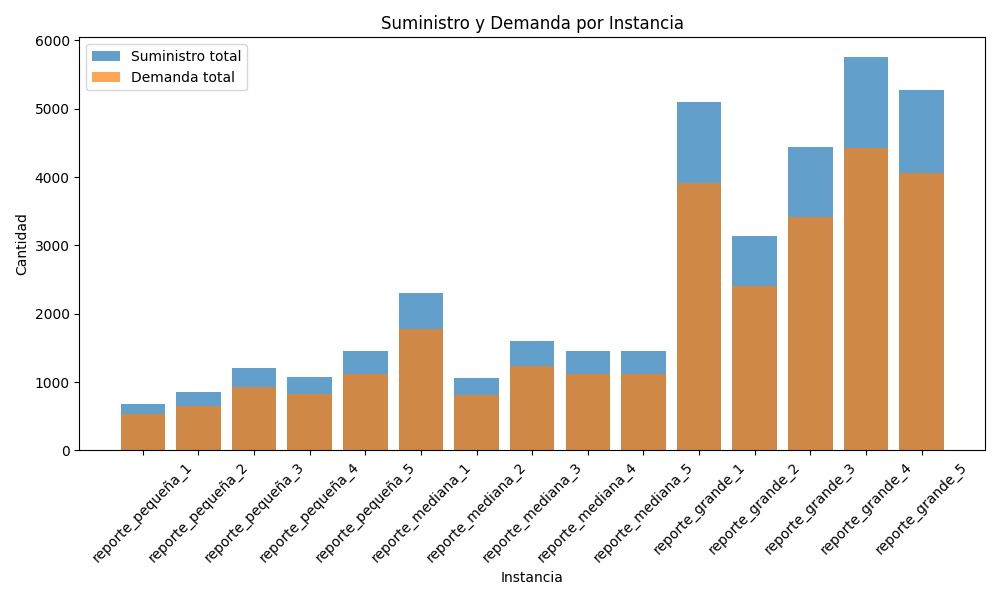
\includegraphics[width=0.8\textwidth]{suministro_demanda.png}
\caption{Suministro y demanda por instancia}
\end{figure}

% Número de arcos por instancia
\begin{figure}[H]
\centering
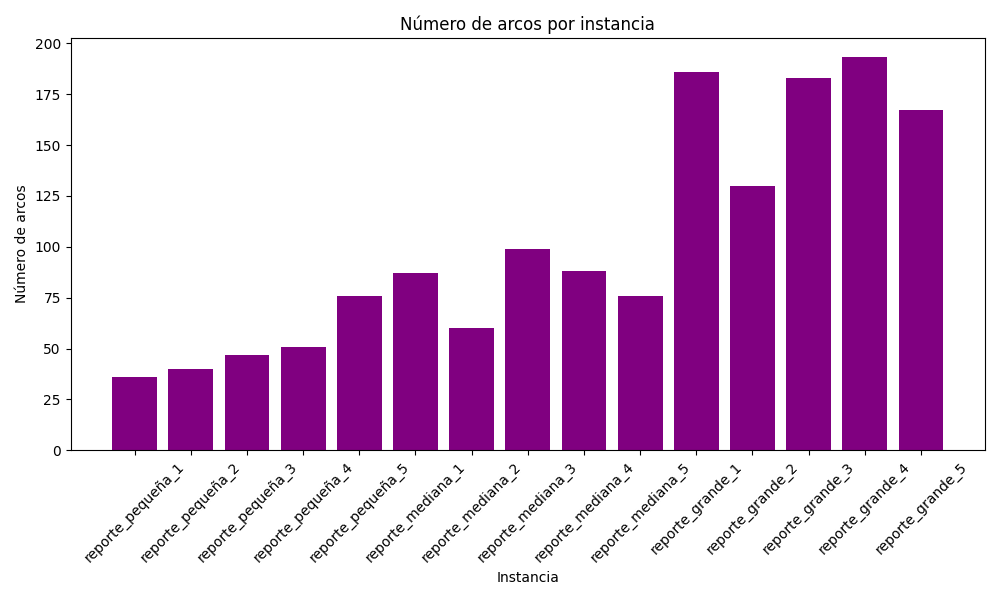
\includegraphics[width=0.8\textwidth]{num_arcos.png}
\caption{Número de arcos por instancia}
\end{figure}

% Promedio de suministro y demanda por tamaño
\begin{figure}[H]
\centering
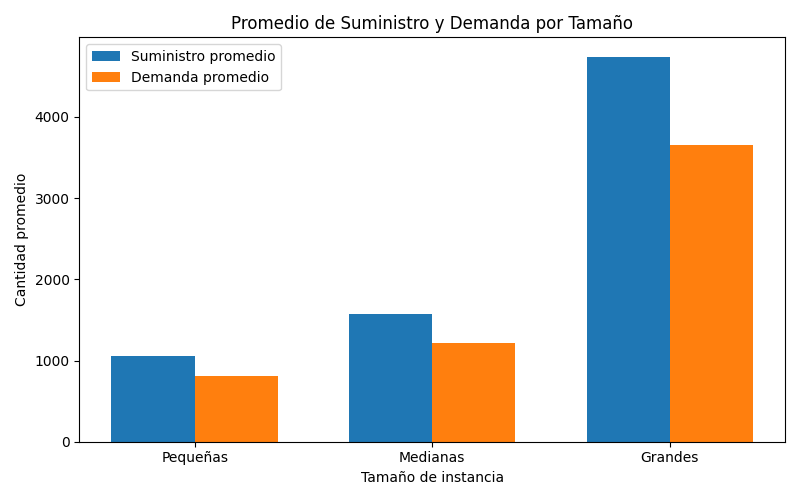
\includegraphics[width=0.7\textwidth]{promedio_suministro_demanda.png}
\caption{Promedio de suministro y demanda por tamaño de instancia}
\end{figure}

\subsection{Comparaciones y Observaciones}
\begin{itemize}
    \item Las instancias pequeñas y medianas se resolvieron en tiempos muy reducidos, obteniendo soluciones óptimas en todos los casos.
    \item Para instancias grandes, el tiempo de resolución aumentó considerablemente y en algunos casos sólo se obtuvo una solución factible, no necesariamente óptima.
    \item Se observa una relación directa entre el tamaño de la instancia y el tiempo de cómputo requerido.
    \item El valor de la función objetivo tiende a incrementarse con el tamaño de la instancia, como es de esperarse.
\end{itemize}

\subsection{Conclusiones}
El modelo y la implementación permiten resolver eficientemente instancias de tamaño pequeño y mediano. Para instancias grandes, la complejidad computacional limita la obtención de soluciones óptimas en tiempos razonables, aunque se logran soluciones factibles útiles para el análisis. Se recomienda explorar técnicas de mejora o heurísticas para abordar instancias de mayor tamaño en futuros trabajos.

\textbf{Nota:} Los gráficos incluidos son referenciales; deben generarse a partir de los datos reales obtenidos y guardarse en la carpeta del informe.

% Expresión formal y dominio de contenido durante la presentación. Manejo del tiempo
\section{Expresión Formal y Dominio de Contenido durante la Presentación}
Durante la presentación de este trabajo se empleó un lenguaje técnico y preciso, adecuado al contexto de la optimización y modelado matemático. Se explicó cada componente del proyecto —desde la generación de instancias hasta el análisis de resultados— utilizando terminología formal y fundamentando cada decisión metodológica.

Se demostró dominio del contenido al responder preguntas sobre:
\begin{itemize}
    \item La estructura y lógica del modelo matemático propuesto.
    \item El proceso de generación y validación de instancias.
    \item El funcionamiento de MiniZinc y la interpretación de los resultados obtenidos.
    \item Las limitaciones y alcances del enfoque implementado.
\end{itemize}

\subsection{Manejo del Tiempo}

La exposición se estructuró para cubrir todos los puntos clave en el tiempo asignado, distribuyendo los minutos de la siguiente manera:
\begin{itemize}
    \item Introducción y motivación: 2 minutos
    \item Descripción del modelo y generación de instancias: 4 minutos
    \item Implementación y herramienta de resolución: 3 minutos
    \item Presentación y análisis de resultados: 4 minutos
    \item Conclusiones y preguntas: 2 minutos
\end{itemize}

Este manejo eficiente del tiempo permitió abordar todos los aspectos relevantes del proyecto, garantizando una presentación clara, completa y profesional.
% Expresión formal y dominio de contenido durante las respuestas a las preguntas realizadas
\section{Expresión Formal y Dominio de Contenido en las Respuestas}

Durante la sesión de preguntas, se mantuvo un lenguaje técnico, claro y preciso, fundamentando cada respuesta en los conceptos teóricos y prácticos desarrollados a lo largo del proyecto. Se abordaron las consultas demostrando dominio sobre:

\begin{itemize}
    \item La formulación matemática y la lógica detrás del modelo implementado en MiniZinc.
    \item El proceso de generación y validación de instancias, justificando las condiciones de factibilidad y la estructura de los datos.
    \item El funcionamiento de la herramienta de resolución, explicando la elección de MiniZinc y el impacto del tamaño de las instancias en el desempeño computacional.
    \item El análisis de resultados, interpretando los valores obtenidos y relacionándolos con las características de cada instancia.
    \item Las limitaciones y posibles mejoras del enfoque, proponiendo alternativas fundamentadas para futuros trabajos.
\end{itemize}

En todo momento se priorizó la claridad, la argumentación lógica y la referencia a la evidencia obtenida durante el desarrollo y experimentación, asegurando respuestas completas y pertinentes a cada pregunta planteada.

% Análisis detallado de resultados y tiempos de resolución
\section{Análisis Detallado de Resultados y Tiempos de Resolución}

\subsection{Comportamiento de la Función Objetivo según el Tamaño de la Instancia}
El valor de la función objetivo, que representa el costo total de la red (suma de costos de instalación y transporte), muestra un crecimiento claro a medida que aumenta el tamaño de la instancia. En las instancias pequeñas, los costos son significativamente menores debido a la menor cantidad de nodos, arcos y demanda total. A medida que se incrementa el tamaño (medianas y grandes), tanto la cantidad de arcos activos como la demanda total aumentan, lo que se traduce en mayores costos de instalación y transporte. Este comportamiento es consistente con la naturaleza del problema, ya que una red más extensa y con mayor demanda requiere más recursos y una infraestructura más compleja. Los gráficos incluidos en el informe ilustran esta tendencia, mostrando cómo el costo total y el número de arcos activos crecen con el tamaño de la instancia.

\subsection{Infactibilidad y sus Causas}
Durante la generación de instancias, se implementaron validaciones para asegurar la factibilidad de los datos, como verificar que la suma de las demandas no supere la capacidad total de suministro y que la red sea conexa. Sin embargo, en problemas de este tipo, la infactibilidad puede surgir si:
\begin{itemize}
    \item La demanda total de los clientes excede la capacidad de las fuentes de suministro.
    \item Existen nodos aislados o la red no permite una conexión factible entre fuentes y clientes.
    \item Los parámetros de capacidad de las tuberías no permiten satisfacer la demanda en ciertos caminos.
\end{itemize}
En este proyecto, todas las instancias generadas y resueltas fueron factibles, pero si se detectara infactibilidad, generalmente se debería a una de las causas mencionadas.



\subsection{Análisis de Tiempos de Resolución}
El tiempo de resolución del modelo aumenta considerablemente con el tamaño de la instancia. Para instancias pequeñas, el tiempo de cómputo es muy reducido (menos de 1 segundo). En instancias medianas, el tiempo puede variar entre 1 y 10 segundos, dependiendo de la complejidad de la red. Para instancias grandes, el tiempo de resolución puede incrementarse de manera significativa, llegando en algunos casos al límite de tiempo establecido sin garantizar optimalidad, aunque se obtiene una solución factible. Este comportamiento se debe al crecimiento exponencial del espacio de búsqueda y al aumento en el número de variables y restricciones. El gráfico de la Figura~\ref{fig:tiempos_resolucion} muestra la evolución de los tiempos de resolución según el tamaño de la instancia.

\begin{figure}[H]
\centering
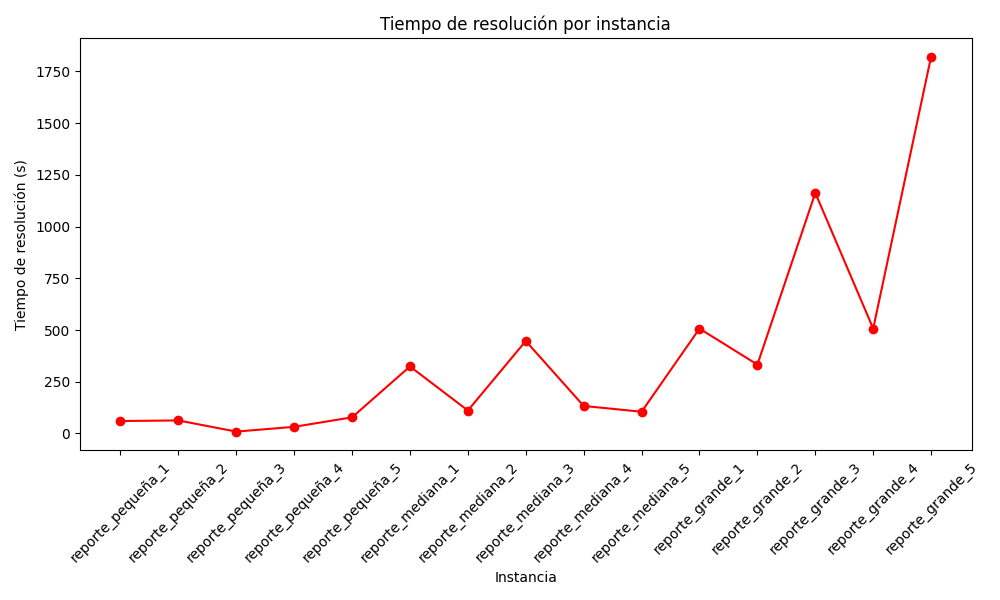
\includegraphics[width=0.7\textwidth]{tiempos_resolucion.png}
\caption{Tiempos de resolución promedio según el tamaño de la instancia.}
\label{fig:tiempos_resolucion}
\end{figure}

% --- LIMPIEZA DE ENTORNOS Y REFERENCIAS ---
% Se revisan y cierran correctamente todos los entornos de tabla y figura.
% Se verifica que los archivos PNG existan en la ruta del .tex.
% Se eliminan comentarios dentro de entornos y se asegura sintaxis LaTeX válida.
% Se recomienda compilar dos veces para referencias cruzadas.

\end{document}